\documentclass[tikz,border=4pt]{standalone}
\usepackage{pgfplots}
\pgfplotsset{compat=1.18}
\usepgfplotslibrary{groupplots}
\begin{document}
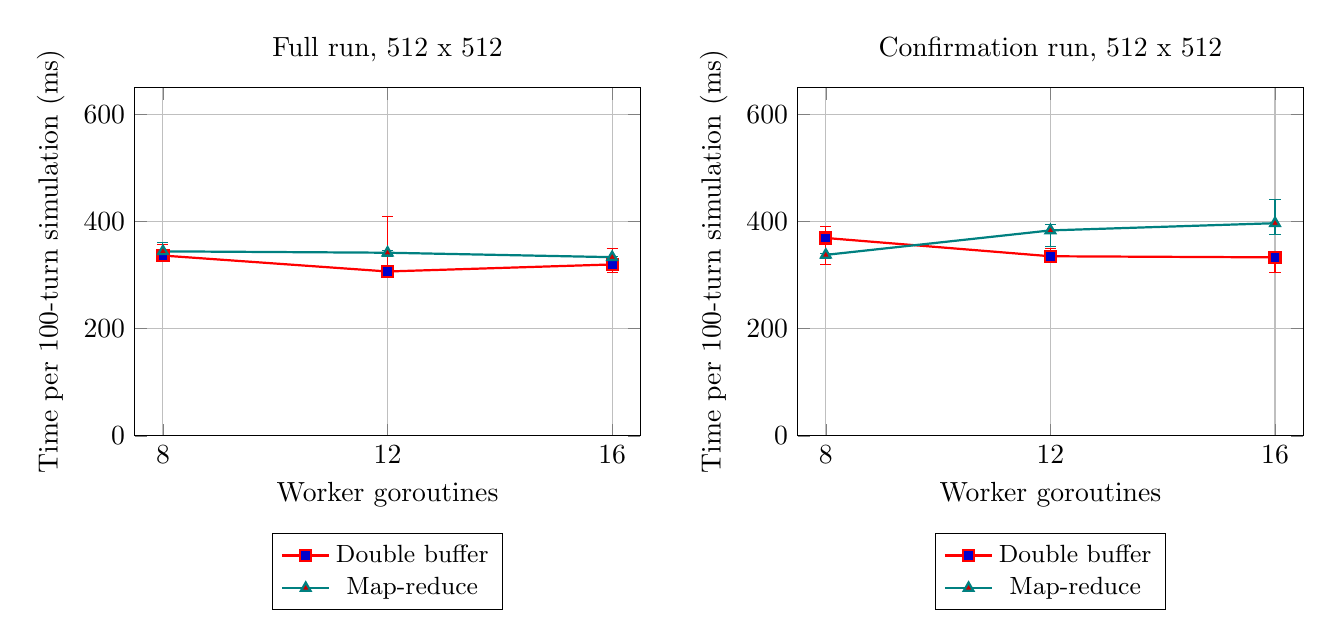
\begin{tikzpicture}
\begin{groupplot}[group style={group size=2 by 1,horizontal sep=20mm},
width=8cm,height=6cm,xlabel={Worker goroutines},
ylabel={Time per 100-turn simulation (ms)},
xtick={8,12,16},xmin=7.5,xmax=16.5,ymin=0,ymax=650,grid=major,
legend style={font=\small,at={(0.5,-0.28)},anchor=north}]
\nextgroupplot[title={Full run, 512 x 512}]
\addplot+[color=red,mark=square*,thick,error bars/.cd,y dir=both,y explicit] coordinates {(8,336.708872) += (0,20.650805) -= (0,11.238813) (12,306.952706) += (0,102.438019) -= (0,2.398778) (16,320.102701) += (0,29.775554) -= (0,14.355457)};
\addlegendentry{Double buffer}
\addplot+[color=teal,mark=triangle*,thick,error bars/.cd,y dir=both,y explicit] coordinates {(8,344.572874) += (0,17.098530) -= (0,5.972888) (12,342.004570) += (0,4.708160) -= (0,7.600044) (16,333.710151) += (0,0.935695) -= (0,8.539246)};
\addlegendentry{Map-reduce}
\nextgroupplot[title={Confirmation run, 512 x 512}]
\addplot+[color=red,mark=square*,thick,error bars/.cd,y dir=both,y explicit] coordinates {(8,369.561407) += (0,20.787395) -= (0,49.684322) (12,335.390539) += (0,13.771664) -= (0,0.826134) (16,333.348905) += (0,5.822073) -= (0,28.560333)};
\addlegendentry{Double buffer}
\addplot+[color=teal,mark=triangle*,thick,error bars/.cd,y dir=both,y explicit] coordinates {(8,337.987227) += (0,3.308601) -= (0,6.057005) (12,383.690146) += (0,10.394999) -= (0,30.305487) (16,397.178233) += (0,43.655483) -= (0,20.616009)};
\addlegendentry{Map-reduce}
\end{groupplot}
\end{tikzpicture}
\end{document}
